\chapter{Introduction}
% 1st sect: GENERAL BACKGROUND & MOTIVATION
A problem occurring in nearly every application of machine learning is the challenge of handling evolving environments, a problem known as  concept drift. Meanwhile, in the domain of big data systems, completely different challenges arise, such as being able to process the volumes of data coming in while meeting decent application response times. The combination of these two problems, the need to adapt the machine learner and simultaneously handling volumes of data, is complex, but common.

Each domain in which this combination of problems are tried to be solved is unique. Each has its domain and requirements that vary in terms of multitudes of aspects such as required throughput, the nature of the changes in the environment, available architecture, and regulation.
Because of this variety in use cases a more fruitful approach to searching for a way of handling adaptation to concept-drifting data should come from the point of view of a case, so the solution can be searched for given some set of assumptions and requirements. 

% which points from the domain will actually be important regarding the discussion will be found out later, these should be changed then.
In this thesis the domain of maritime is used as a starting point, and facilitating updates to deep learning models solving problems such as traffic forecasting and navigation as the goal. The domain in question is characteristic in the especially large volume of data coming in in form of sensor messages, and the relative slowness of vessel traffic in comparison to computing. Other points from the domain of application considered are the low quality of incoming data, heterogeneousness of data sources, and complexity of the machine learning models needed; most of these are tailored to the specific case of, for instance, weather routing.

Traditionally, works addressing the problem of concept drift largely focus on how to build a model that is able to adapt to the environment changes. This thesis can, from this perspective, also be seen as a systems approach to concept drift. If a model is taken as given, it is discussed how the system organization would be able to make sure the model stays accurate. This systems perspective aims to find a solution that not only works, but also takes into account best practices known from the field of designing big data systems. From the lessons learned there it is especially aimed for a solution that is simple and mature enough to be applied to a real-world scenario.

% 2nd section: RESEARCH Q'S, METHODOLOGY, RESULTS SUMMARY

% outline
% main question
% exact definitions of main question
% sub-questions
% note on methodology (literature based but not systematic, non-empirical)
% results summary

% comment: the sentence on the model is a little vague, tailored means that it is made for the case not just taken from somewhere else. I'm unsure what words to mention on the model here.

The thesis at hand will revolve around one main research question, under which some further specifying sub-questions will be investigated. The main point of investigation is the following:

\begin{center}
    Given the domain context and the models used, how to organize a workflow for efficient updating of the models in order to meet the demands posed by the use case?
\end{center}

As further elaboration, by updating the model it is meant that the model parameters are changed. By efficient we mean efficiency relative to the data volume, not relative to computing resources. This means that an average high performance cluster having the processing power of ... data here ... is assumed and the target is to be able to utilise that to be able to handle as much data in as little time as possible. The model used is assumed to be a complex deep learning model tailored to its specific task, operating in batch mode. Domain context and use case are dissected in section 2.3.

The secondary research questions considered as implications of the primary one are the following:

\begin{itemize}
    \item How much human intervention is required for maintaining the updating schemes; what are the possibilities of automating these workflows?
\end{itemize}

% add more implication-type questions later...
% add paragraph on results here later...

As a note on methodology, the investigation in its entirety is based on literature. Conducting a systematic literature review would be beyond the scope of this thesis, so only material directly relevant regarding the specific set of requirements is taken into account. Testing the various approaches in practice is also beyond scope; the empirical investigation of these findings is left to future works. This limits that both the set of options considered to those already used in the problem domain and the evaluation to analyzig the thoroughness of existing evidence in literature.

% 3rd section: CHAPTER ROLES
% ways of automating might be out of scope, can be deleted if it does not fit in
% if the result is so that multiple can be good then change chap 4 description to state that the systems applying the max two best seeming options are presented.

The rest of this thesis is organized as follows:

Chapter 2 presents the necessary background knowledge to the reader: an overview of the general organization of a big data system, definitions in the field of machine learning model updating, and an introduction to the maritime domain. Chapter 3 analyzes the various model updating approaches presented previously and discusses which approach would be most useful given the context of the case. Then, ways of automating the optimal-seeming approaches are shortly discussed. 

Chapter 4 synthesizes the findings above and presents an abstract overview of the system that would apply the optimal updating workflow. In addition it is discussed how certain these findings are given the quality and thoroughness of the literature used. The paper is concluded with discussion on the applicability of the results achieved to similar problems from different domains.

\chapter{Overview on large-scale machine learning systems for maritime}


\section{On big data systems}

% MLOps is a term that should be used / mentioned somewhere

% current main concern for this sect: I state out a lot of facts without giving a reference -> the fine line between common knowledge and what needs backing...

\subsection{The high-level components}

% is this section necessary?

The steps that most large-scale machine learning systems compose of are displayed in the following figure: 

% how do I properly cite the google cloud developer guide?
% the figure is too small... -> not very readable
\begin{figure}[ht]
%\begin{figure}[tbh] t= top, b = bottom, h=here
\ \newline
\begin{center}
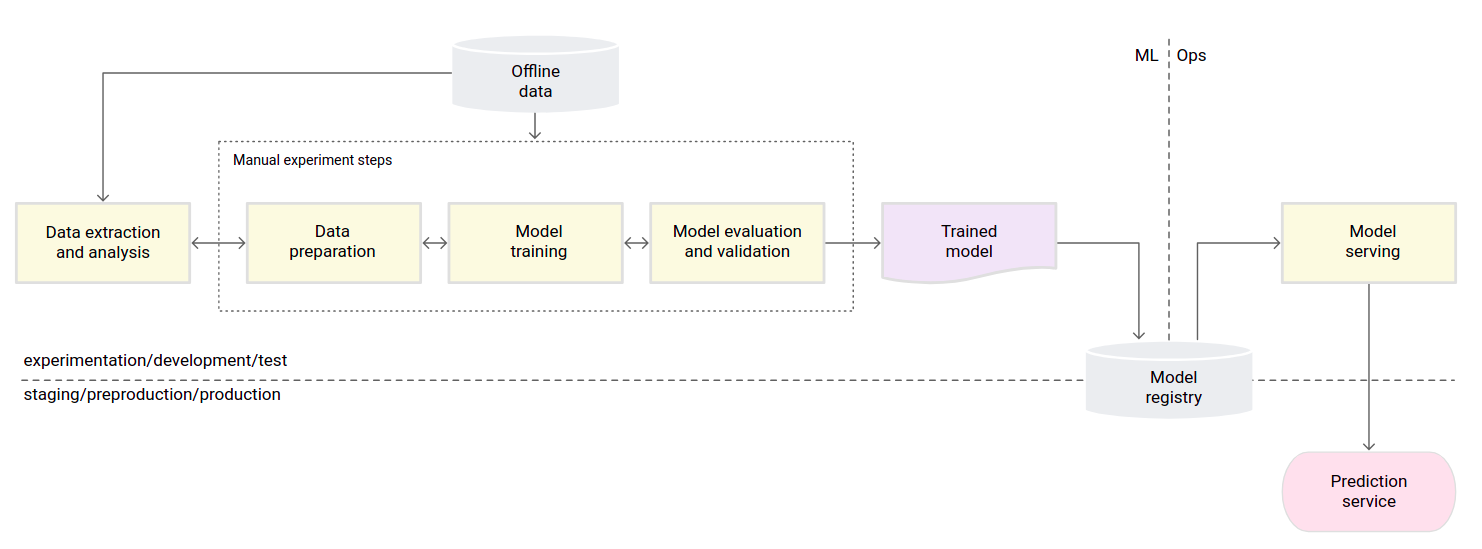
\includegraphics[width=0.9\textwidth]{simplegoogle.png}
\caption{Abstract components of a big data analytics system. From Google Developer MLOps guide \cite{googlemlops}.}
\label{simplepipeline}
\end{center}
\end{figure}


While the steps above represent a coarse abstraction, hiding away feedback loops and the multitudes of ways each part can be implemented, most contemporary big data systems implement all of the following steps:

\textbf{Data extraction}: this component is responsible for handling the incoming data. Usual forms of data are either web logs, coming in from a server, or IoT data, coming in from sensors that are often geographically distant from the data ingesting component.
% that data is usually web logs or sensor requires a reference?

In big data systems incoming data is represented either as batches, meaning chunks of data coming in at certain intervals, or as a stream, meaning that individual data records are coming in constantly. The main advantage of using a batch representation is known to be increased throughput%(find citations here)
, while stream processing allows smaller end-to-end latencies. %(find citations here)
% the usually interpreted as stream or batch needs a ref too?

To mitigate the tradeoff between throughput and latency, a popular solution is called the lambda architecture. This reference architecture has a processing unit for both batch and stream data with the stream component, so-called speed layer, handling requests for the data not yet processed by the batch layer \cite{beatingcap}. While this approach is widely accepted to solve the problem of handling highly voluminous data fast and mitigating human errors by allowing restarting the speed layer any time without losing data \cite{lambdakappa}, the architecture has faced criticism for being redundantly complex and forcing the data ingestion code to be written twice \cite{questioninglambda} \cite{uber} \cite{facebook}. As an alternative, the kappa architecture has been proposed, only composing of either a batch or a stream processor, usually the latter \cite{questioninglambda}. This mitigates duplication, but retains the tradeoff with throughput and latency \cite{lambdakappa}.

\textbf{Data preparation}: This step encompasses the processes of data cleaning, transformation, and feature engineering. Data cleaning refers to operations identifying and removing faulty data, such as values that are missing or are clearly impossible. Data transformation and feature engineering are used interchangeably, both meaning processes that transform data into a format that the models used can process. A popular example in this is the mapping of plain text into word count matrices \cite{dapbook}.

While the data preparation step is often overlooked in literature,
it is a both challenging and crucial part of the system as preprocessing commonly takes up a majority of the total end-to-end latency of a machine learning system \cite{adaptivelearningsystems}. As for systems design, the most relevant decision to make is whether to clean data before it is saved to the data storage, or only when it is  needed for training. The main benefit with the first approach is that data only needs to be cleaned once, while the latter allows processing data for different models in different ways.
% the two approaches and their tradeoffs need a ref...
% the how many % of time preprocessing takes needs a ref... i got one somewhere...

\textbf{Data storage}: Interpreted in the figure as offline data, the data storage is used to save the data that is needed for model training. The most often used storage methods are called data warehouses and columnar databases. Due to the volume of the data, the storage is either cleared often completely or only a small part of the data is archived.
% data archival needs a ref.
% popular ways of implementing data storage too!

\textbf{Model training}: This component is responsible for training the model, which means tuning the model parameters in a way that it fits to the distribution of the incoming data in order to make accurate predictions from data coming in during operation.

The training conducted can be done from scratch, meaning that the same instance of the model has not been trained before, or in cases of using adaptation-capable models, the models can be updated. Details on model updating or retraining are discussed below.

As for infrastructure, training can be conducted in a central or federated manner. Centralized training, often run in a cloud data center, can run either on one machine or distributed across multiple cores by splitting the model or the data to parallelize the training \cite{iotsurvey}. As the amount of data is large, high-performance computing (HPC) clusters and modern general processing units (GPU) are used to reach required latencies \cite{iotsurvey}. Federated approach refers to an internet of things setting where the training is conducted in the edge devices of the IoT network. This aims to solve the issues of moving privacy-sensitive data across the network and being able to adapt to the unique environments of each data source \cite{iotsurvey}. As in the maritime context the data is neither highly private or has differing environments in different sensors, the federated approach is not considered further in this work.

\textbf{Model evaluation and validation}: In this stage the model is tested and adjusted in various ways. For testing, usually various model metrics such as accuracy for classifiers and error statistics for regression tasks are checked \cite{iotsurvey}. These numbers can also be compared against other models, possibly models already in operation \cite{googlemlops}. Also testing different data sets and checking compatibility with the rest of the system is conducted at this stage \cite{googlemlops}.

In addition to testing, models are also optimized for the infrastructure that they are being deployed on. This can include, for example, various performance optimizations, or in case of constrained memory, model compression \cite{iotsurvey}.

\textbf{Model registry}: is a centralized storage for the trained models. 

% need a reference here as well...

\textbf{Model inference}: edge fog cloud here marked in the figure as 'prediction service', this component contains the trained models that are used for answering application requests. These requests can require data statistics, computed with conventional data analytics, or predictions made by machine learning models.

The most important design decision to make for this component in the sensor data scenario is where to deploy the models, in the cloud, a cloudlet or 'fog', or on the edge. Cloud means that the model is deployed in a data center and edge refers to models being deployed in the IoT devices. Fog refers to the in-between solutions: 

OCF is The Open Connectivity Foundation. add below + the proper source

The definition of fog computing is the following, as stated by the the OCF (in \cite{fogsurvey} reference [42]): “Fog computing is a horizontal, system-level architecture that distributes computing, storage, control and networking functions closer to the users along a cloud-to-thing continuum.” (but not only entirely to the edge). Or, put differently by \cite{fogsurvey} for a clearer mental image: "The Fog is a Cloud closer to the ground."

\subsection{Best-practice design principles}

%\cite{designprinciples}: most important things are system stability with fluctuating data quality, scalability, minimal human intervention

%\cite{facebook}: ease of use, performance, fault-tolerance, scalability, correctness

%\cite{storm@twitter}: scalable, resilient, extensible, efficient, easy to administer

%\cite{uber} always a tradeoff between requirements, quick iteration for improvements, quich scaling in hardware

%\cite{millwheel}: fault tolerance, scalability

%--> synthesized there is scalability, resiliency for faults & environment changes, easy to improve the system 

%also some genaral principles on bd systems. Tradeoffs is big: usually to achieve better results in some respect simplicity is sacrificed. The goal is to do complex in right places where real benefits can be received, and keep it simple elsewhere. Also point on this is that the big mature big data systems stated that simplicity or ease of use or maintainability, basically variants of simplicity, is the most imporant trait or one of the most important

In order to design a working big data system, taking into account lessons and best practices learned in the past greatly increases the chances of succeeding in operation. In general, as stated by the authors of \cite{uber}, in systems design everything is a tradeoff: every design decision taken to improve the system in some respect inevitably will degrade quality in another respect. At its simplest, for instance, improving the systems throughput by adding ... (what?) in a way adds complexity, meanwhile sacrificing simplicity.

The most mature big data systems as of date have each evolved on their own but despite that have identified quite similar best practices, that should be preferred no matter the field of implementation. In each system compared, Google MillWheel \cite{millwheel}, Facebook \cite{facebook}, Twitter storm \cite{storm@twitter}, the M6D ad targeting engine \cite{designprinciples}, and the Uber system \cite{uber}, there is a slight variance in emphasis of importance and naming of each one, but in general the following traits were deemed the most important across all systems:

\begin{itemize}
    \item \textbf{Ease of using and improving}: while others named this as 'ease of use', others named 'easy to administer', 'easy to improve' or 'minimal human intervention', in general all terms refer to how usable the system is. Its operation should be effortless, but at the same time, improving it should be quick, as this enables fast adaptation to ever-changing application needs. In addition, modularity is in this respect important as it enables iterating individual modules, and simplicity in general makes a system both usable, and easier to update.
    \item \textbf{Scalability}: Scalability was named as one of the most important trait to favor across all systems descriptions listed. Scale is at the core of the nature of big data, and with expectations of the amount of data doubling every x years (need a reference for this), it is reasonable to constantly be prepared to handle ever-growing quantities of data. This can be achieved through various solutions of distributed computation, or making adding more hardware to the system as seamless as possible.
    \item \textbf{Resiliency}: Under this umbrella term fit both the terms fault tolerance and resiliency to changes in the operational environment. With big systems consisting of multitudes of components and different types of infrastucture, individual parts of the system failing is a very common occurence. In addition, in terms of the machine learning conducted in the systems, the models should be able to perform in a stable manner, meaning that the prediction accuracy variance should stay small despite minor changes in the incoming data, or other changes in the environment.
\end{itemize}

\section{Model updating approaches: terminology}

% to-do: add adaptive learning approaches to the first subsect and remove subsectioning

% this section: I should have more sources and double-check that I got the definitions correct.

% mention the types of adaptive learning earlier

% find reference to "There are two broad ways of retaining knowledge"

% Knowledge retention is a self-invented term and should be replaced with a better one.

% online learning is kind of synonymous to stream processing and can (?) be taken as given. define it here or elsewhere, in systems possibly.

%define real and virtual drift?
%model specific and model independent adaptation could be a good divide
%conceptdriftsurvey was the first to use the term(lecture)

In machine learning based systems, the term \textbf{knowledge retention} means extending the span of time of a machine learning model from months to years while preserving its performance. Here ''knowledge'' means the model parameters that resulted from training a machine learning model of a specific machine learning task. There are two broad ways of retaining knowledge. Firstly, one can use a model for a specific task in an environment that is shifting over time. This is called \textbf{adaptive learning} \cite{conceptdriftsurvey}. Secondly, a model can be used in multiple tasks; the knowledge gained from training for one task can be transferred to similar problem domains. This is referred to with \textbf{transfer learning} \cite{lmlsystems}.

The paper at hand is dealing with the problem of adaptive learning. However, as terms can be easily confused and misunderstood, some terms regarding transfer learning are defined next.

\textbf{Lifelong learning} is a machine learning paradigm of ''learning many tasks over a lifetime from one or more domains'' \cite{lmlsystems}. This means that the knowledge gained from one task is processed in a way that it can be applied to a related task. As of date lifelong learning is implemented for simple classification tasks, and the new tasks are usually introduced by including unseen classes of data for the testing data set \cite{lmlinneuralnets}. A new environment could also perhaps be interpreted as a new task, but as the paradigm is currently still new and tackling very simple problems \cite{lmlinneuralnets}, it is too early for its adoption to a real-world scenario with complex models.
% stability-plasticity is a transfer learning problem. omit.
The general challenges arising in knowledge retention are the following. Especially within transfer learning \textbf{the stability-plasticity dilemma} is central. This refers to the need of finding an optimal balance on when to retain the old knowledge (stability) and when to replace it with new insight (plasticity) in order to perform well in predicting for both the old tasks seen and the new ones emerging later. Overdoing plasticity, i. e. replacing old parameters too easily may sometimes lead to \textbf{catastrophic forgetting}, which means that the ability to predict accurately for the old tasks is lost completely or for a big part.

% add: that the only legitimate option to drift mitigation is retraining, which is cpu-heavy.
Within adaptive learning the central problem to address is called \textbf{concept drift}. This means, in technical terms, that ''the relation between the input data and the target variable changes over time'' \cite{conceptdriftsurvey}. This is usually the result of changes in the environment in which learning is conducted. For example, in the maritime domain, it is possible that over the years vessels' speeds increase, and as a result the old trajectory forecaster predicts systematically false future locations for vessels.

The concept drift can include in itself a need for balancing stability and plasticity, depending on the use case. In autonomous cars, for example, an adaptive learning algorithm could change its predictions based on shifts in lighting and terrain conditions, but it should still be able to operate in the conditions it has seen before the changes \cite{conceptdriftsurvey}. In contrast, in maritime, it is not necessary for the models to perform well in an environment of the past after marine traffic conditions have shifted over time.

% maybe add here the definition of feature drift: "A feature drift occurs when a subset of features becomes, or ceases to be, relevant to the learning task [10]" (from mlflorstreamingsurvey) -> feature evolution will be a rare occurence in vesselai, can be omitted? also streamminingchallenges stated that feature drift is an important problem to address!

% maybe add: also hyperparams need to evolve! \cite{mlflorstreamingsurvey}

% maybe add: there is gradual and abrupt drift \cite{streamminingchallenges} \cite{conceptdriftsurvey}

In the following section the ways of mitigating the effects of concept drift whilst maintaining performance on old tasks, if necessary, are presented.

The ways of doing adaptive: retraining, incremental learning, online learning. Then there was the ways of preserving old data and re-feeding it to models. Then there are the ensemble learning techniques, putting models to sleep state, blind&informed adaptation, ways for feedback mechanisms
% ! zliobailte's concept drift survey (not conceptdriftsurvey but the 2nd): incremental learning is not related to adaptation, it is a different domain! do not confuseeeee
-> there are a lot of ways, many ways to classify the ways also. Make more sense of what each means and how they should be presented. Find more sources than \cite{conceptdriftsurvey} to find more insight.

definitions
 retraining: taking a new instance of the model and completely training it again from scratch
	    incremental learning: a model is trained with each batch coming in from a data source and updated after each training. a way of doing adaptive learning.
	    online learning: the model is updated with each data entry coming in from a data stream and is simultaneously constantly in operation. a way of doing adaptive learning.
	    ensemble learning: adapting through predicting with a combination of models

% add here: in order to implement adaptive learning, a few new components need to be introduced. Then display the more complex system description and explain with emphasis the trigger and monitoring

% iotsurvey has a decent seeming sect on the monitoring stuff

\section{Context and requirements from the maritime domain}
% maritime is global
Maritime as a domain of application for a sensor-based machine learning system differs in a few ways from others. The most obvious difference is its global nature: while other spatial domains such as smart cities also have to take geographical distribution into account, maritime is special as it encompasses all of what the earths' surface mostly is covered by: the seas. 
% maritime is extreme heterogeneous data

As another characteristic, equally to the area that is operated in, the amount of traffic is large, which results to data volumes exceeding even what is conventionally noted as big data. Due to international regulation vessels have to send update signals of their status from every few minutes to every two seconds, depending on their speed and course \cite{maritimeinformatics}. With approximately 100, 000 ships sailing the world oceans daily \cite{maritimeinformatics}, this leads to several billion messages sent each day. To this exceptional amount of data we refer to as \textit{extreme-scale data} in this work. In addition to this, in order to provide valid maritime intelligence, other types of data such as geographical information and weather reports are needed \cite{D1.1}. Therefore, the data is not only highly voluminous, but also heterogeneous, coming in both static and dynamic forms at different velocities.

% lack of speed in terms of vessels
Added to scale, another specific of this context is speed, or more specifically, the lack of it. Depending on the size and type of the vessel, it takes from minutes to up to an hour to change course. This means that for machine learning services in this domain the acceptable end-to-end latencies are measured in seconds, even minutes. This differs greatly from other sensor system applications, where latencies are usually measured in the order of hundreds of milliseconds (e.g. \cite{anomalysystem}, \cite{facebook}, \cite{edgelatency}). This means that striving for instant response times is redundant, even of detriment, as prioritizing latency inevitably would introduce the need to make compromises in other respects, such as prediction accuracy.

% AIS intro
The main data source, the status signal data sent by vessels, called \textit{automatic identification system} (AIS) data, also has its specialities. AIS is a form of sensor data and has two types: static messages containing information such as name, destination and ship characteristics, and dynamic messages with information on the vessels' location, speed, heading, and rate of turn. The challenge with AIS data is both its highly fluctuating reporting intervals and especially its unreliability.  Things such as manually written destinations, faulty timestamping, lack of universal identifiers, misreported locations, and even illegal traffic camouflaging their operations, make identifying and correcting erroneous data both difficult and computationally expensive. In addition to faults in the data itself, another layer of error is added by the traffic system: factors such as busy areas where part of messages go lost because of overloaded receivers and vessels shutting off transmitters in fear of smugglers bring additional entropy to the data \cite{maritimeinformatics}.

% pilots
The goal of the project studied, called VesselAI, is to provide the following four pilot services to users: route forecasting for traffic monitoring and management, design of optimal ship energy systems, operating autonomous ships in short sea transport, and weather-optimized routing for long-distance voyages. In addition to this, the more abstract goals are to find a system that is suitable for both managing extreme-scale data and enabling the models to run in production over extended periods of time. The goal is also to be able to fully utilize the most modern high performance computing infrastructures in an optimal way, and develop new machine learning methods \cite{D1.1}.

% requirements derived from above
With this context and goal specification in mind, the following system goals and challenges can be stated. The general goal is to be able to provide accurate predictions not in an instant, but still in a time-constrained manner. Two main challenges arise from the combination of context and required services that most pressingly need to be addressed to reach this goal. Firstly, the nature of data used sets high demands on the training part of the workflow: storage, preprocessing, and training. Secondly, given the environment of operation, concept drift identification poses a challenge. As data quality is low, distinguishing drift from noise is hard, especially as it can be expected that the drifts will be more of the gradual type; abrupt drifts will likely be encountered only within subsets of the data. The time spans of vessel operating mean that the prediction correctness is known only after days, which means that the problem of delayed labels is very present in the domain.

How to deal with these challenges, in order to build a system able to meet its requirements, is the primary topic of inspection in the following chapters.

%outline:
% 1st paragraph: maritime specifics: geo distr, volume, vessel slowness
% 2nd paragraph: data is heterogeneous and error-prone
% missing data due to lots of traffic -> receivers dont take in everything. senders turned off bc smuggling

% 3rd paragraph: pilots n abstract aims
% the project
%	the pilots I-V: what each one aims for
%		these ml problems are difficult
%	abstract aims
%		deal with extreme scale data
%		facilitate continuous learning
%		utilize modern HPC

%data thoughts
%		static and dynamic, fast and slow paced
%			examples: map data, weather data, sensor data
%	many models only need a small fraction of the data


% combine these: the requirements.
% we want accurate solutions to hard problems not instantly, but it should not take forever either
% security is no obstacle
% obstacles to reach this
% there's a big need for data preprocessing (emphasis on workflow efficiency)
% concept drift is gradual large scale abrupt only in subset of data (napa example: vessels start anchoring somewhere)
% concept drift: noise vs drift is hard to distinguish bc error data
% correct labels to data come delayed, talking about days to couple weeks. hard to get labels also is possible. mention delayed labels


\chapter{Analysis of model updating approaches for batch learning}

\section{Updating approaches}

The feedback mechanisms issue: is it possible to train supervised with historical data and then operate without performance feedback?

include also here: data cleaning

central vs federated learning: learning location

the approach of doing adaptive learning in a unsupervised / semi-supervised setting

Here: give the +'s and -'s of each approach. This information on how knowledge retention is likely to be applied affects the discussions on the other things in consideration

blind mechanisms

+ no need for a feedbacck system

identifying concept drift approaches

+ more accuracy compared to blind methods \cite{conceptdriftsurvey}

- a feedback mechanism needs to be in the system

online learning

- no way for abrupt adaptation, only gradual \cite{conceptdriftsurvey}

ensemble

+ a mature approach for the problem \cite{mlforstreamingsurvey}

approaches: stable&reactive models, weighted average, model sleeping \cite{conceptdriftsurvey}

data window comparisons

- old data needs to be stored and takes up lots of memory \cite{conceptdriftsurvey} -> probably not applicable

combinations of approaches that are not researched a lot -> immature

\begin{itemize}
    \item concept drift detection + delayed labels \cite{mlforstreamingsurvey}
    \item transfer learning + online learning \cite{mlforstreamingsurvey}
    \item adaptive learning + delayed labels \cite{mlforstreamingsurvey}
\end{itemize}

HERE: initial hunches I have from going through literature on coping with concept drift

ensemble seems popular and efficient

ensemble literature general impression: every approach is stated to be empirically better than the ones compared to. Should find literature comparing them, not presenting something, maybe. Single-model approaches are used as baselines that are compared to, that are definitely worse than all the ensemble approaches.

things that came up a lot
maloof
littlestone
michalski
algorithms: STAGGER, AQ-PM, AQ11-PM, AQ11-PM+WAH. DVM
ensemble diversity
pruning
bagging and boosting

single model approaches
many talk about incremental learning being like a synonym to single model adaptation? is this true? many words are vague in the topic so maybe just choose a definition and start using

%\section{system architecture}

to discuss here: given the model updating approach deemed best for the case, what should the system be like on an abstract level?

\begin{itemize}
    \item where to do data cleaning - maybe too much given the amount of to-discuss here already? \cite{mlforstreamingsurvey} has a good sect on this if this will eb considered
    \item algorithm performance feedback mechanism (was presented as a thing to take into account in \cite{streamminingchallenges})
\end{itemize}

\section{Automating model updates}

discuss here: edge v couldlet v fog v cloud for inference, then also should training be central (hpc) or more distributed

+ and - for fog, from \cite{fogsurvey}

+'s that matter: saves bandwidth, mitigates problems with hostile areas that have fragile net connections (fog is stated to be fundamental in solving this problem), has reached a good enough maturity

+'s that do not matter: saves time (in range 66-302 ms), is somewhat more private, context awareness: able to adjust to location is probably not something the models are able to benefit from because edge training is most likely not computationally feasible

-'s: adds compexity by distribution and heterogenity: " imposes non-trivial orchestration issues", cloud is more energy efficient (fot this check [120] from \cite{fogsurvey}),

so: fog has drawbacks in complexity that are not acceptable considering that the advantages gotten with it are largely irrelevant.

\chapter{The systems application}

i e the results i get

\chapter{Conclusion}

add here applicability of these conclusions to other systems.

could add here: that the results gotten could not be validated empirically as the scope and level of this thesis will not allow for a thorough experimental inspection.

also add maybe here that the literature on the topic is so vast and quickly evolving that it is possible that the subset of existing literature that I have gone through somehow conveys things in a non-objective way. This is unlikely however.
